% fig12_bluemax_pairs.tex — BLUE-MAX 8 atoms: correct integer (PASS) vs
% negative-control wrong integer (FALSIFIED). Paired bars per atom, log-y so the
% integers 2..22589 all fit; the +-1 gap is what the deterministic rubric pins.
% Compiled by the paper Makefile via `make figures` (pdflatex on the snippet).
%
% Data provenance (NO fabrication; commons @D g3) — Appendix F (app:bluemax),
% Tables tab:app:bluemax / tab:app:bluemax:neg (PR #1102). Each pair is the
% registered SUPPORTED-FORMAL integer vs its matched _NEG control (true +-1):
%   q_star_constant                     5  (PASS) vs 6     (FALSIFIED)
%   bosch_hale_gamow_factor             3  (PASS) vs 4     (FALSIFIED)
%   solenoid_axis_bz_half_factor        2  (PASS) vs 3     (FALSIFIED)
%   pb11_reactivity_moment_e6_scale_exp 6  (PASS) vs 7     (FALSIFIED)
%   sigma_v_dt_e18_scale_exponent       18 (PASS) vs 17    (FALSIFIED)
%   pb11_resonance_kev_doubled          296(PASS) vs 297   (FALSIFIED)
%   pb11_quadrature_nodes               600(PASS) vs 601   (FALSIFIED)
%   pb11_gamow_eg_kev                   22589(PASS) vs 22590(FALSIFIED)
%   8/8 positives |Delta|=0 SUPPORTED-FORMAL; 8/8 controls |Delta|=1 FALSIFIED.
%
% Manual single-shot compile (debug):
%   pdflatex -interaction=nonstopmode -halt-on-error fig12_bluemax_pairs.tex
\documentclass[border=4pt]{standalone}
\usepackage{tikz}
\usepackage{pgfplots}
\pgfplotsset{compat=1.18}
\begin{document}
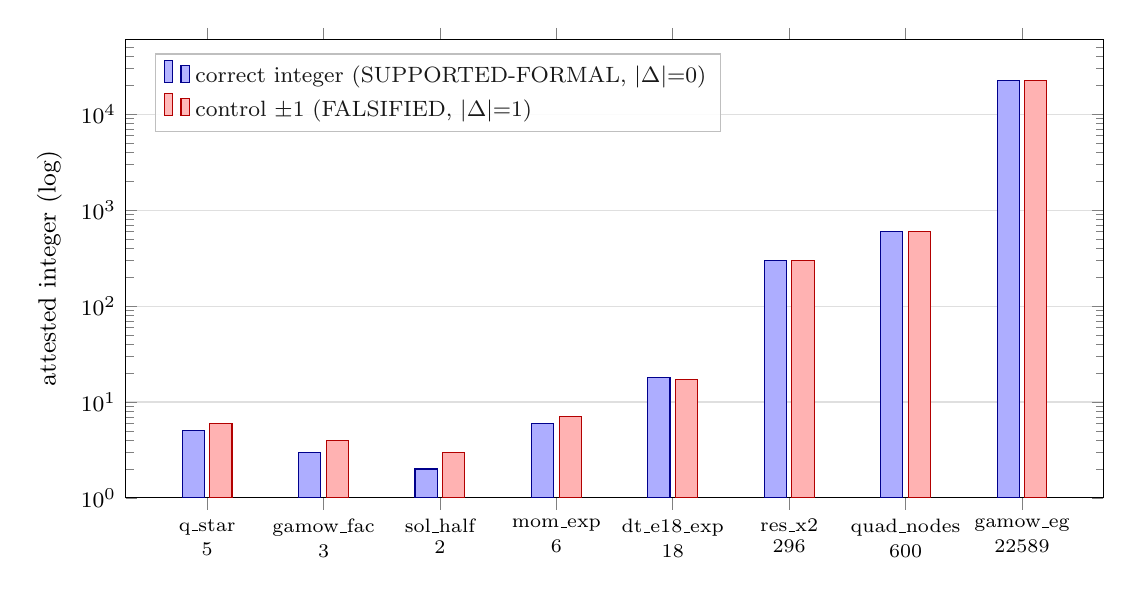
\begin{tikzpicture}
\begin{axis}[
  width=14cm, height=7.4cm,
  ybar,
  bar width=8pt,
  ymode=log,
  log origin=infty,
  ymin=1, ymax=60000,
  ylabel={attested integer (log)},
  symbolic x coords={qstar, gamow, solhalf, momexp, dtexp, res, nodes, eg},
  xtick={qstar, gamow, solhalf, momexp, dtexp, res, nodes, eg},
  xticklabels={%
    \shortstack{q\_star\\\scriptsize 5},
    \shortstack{gamow\_fac\\\scriptsize 3},
    \shortstack{sol\_half\\\scriptsize 2},
    \shortstack{mom\_exp\\\scriptsize 6},
    \shortstack{dt\_e18\_exp\\\scriptsize 18},
    \shortstack{res\_x2\\\scriptsize 296},
    \shortstack{quad\_nodes\\\scriptsize 600},
    \shortstack{gamow\_eg\\\scriptsize 22589}},
  x tick label style={font=\scriptsize,align=center},
  tick label style={font=\footnotesize},
  label style={font=\small},
  ymajorgrids,
  grid style={gray!25},
  enlarge x limits=0.10,
  legend pos=north west,
  legend cell align=left,
  legend style={font=\footnotesize,fill=white,fill opacity=0.9,draw=gray!50},
]
% correct integer -> SUPPORTED-FORMAL (PASS, blue)
\addplot[draw=blue!55!black,fill=blue!32] coordinates {
  (qstar,5) (gamow,3) (solhalf,2) (momexp,6) (dtexp,18) (res,296) (nodes,600) (eg,22589)
};
\addlegendentry{correct integer (SUPPORTED-FORMAL, $|\Delta|{=}0$)}
% negative control wrong integer -> FALSIFIED (red, true +-1)
\addplot[draw=red!70!black,fill=red!30] coordinates {
  (qstar,6) (gamow,4) (solhalf,3) (momexp,7) (dtexp,17) (res,297) (nodes,601) (eg,22590)
};
\addlegendentry{control $\pm1$ (FALSIFIED, $|\Delta|{=}1$)}
\end{axis}
\end{tikzpicture}
\end{document}
